\subsection{Typer af Robotter}

Robotter kan klassificeres på forskellige måder afhængigt af den opgaver de udføre, miljøet de gør det i og design og autonominiveau. Af de kategorier der er beskrævet i \cite{ISO2021ISOVocabulary} og \cite{IFR2023World2023} er der to, for projektet relevante, kategorier.

\paragraph{Industrirobotter} Industrirobotter er automatiserede og programmerbare maskiner, der bruges i industrielle miljøer til opgaver såsom samling, svejsning og malerarbejde \parencite{IFR2023World2023}. Industrielle robotter kommer i alle størrelser men kræver til forskel fra de andre kategorier en masse infrastruktur omkring dem. Det kan fx være indhegninger for robot arme som den på \ref{fig:irb7710pic}. De skal dermed ikke tage højde for mennesker og bruges ofte til at udføre opgaver der er for dyrt at ansætte folk til \parencite{ABB2023IRBSeries, ISO2021ISOVocabulary}. 

\begin{figure}[H]
    \centering
    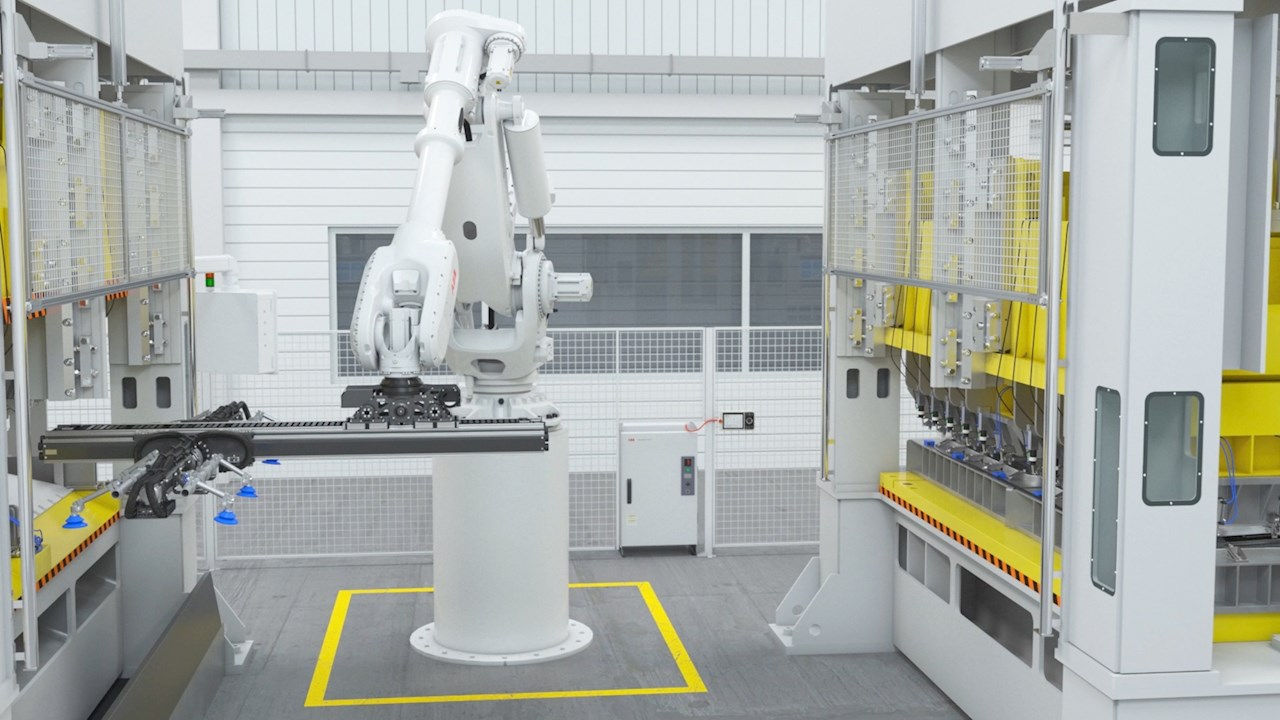
\includegraphics[width=0.6
    \textwidth]{Sections/2 Problemanalyse/Media/irb7710.jpg}
    \caption{IBR-7710 robotarm fra ABB \parencite{ABB2023IRBSeries}}
    \label{fig:irb7710pic}
\end{figure}
\textit{Eksempel:} ABB's IRB-robotter, serien indeholder mange forskellige størrelser af robotter. På figur \ref{fig:irb7710pic} ses 7710, som er i den store ende og har en løftekapacitet på op til 500 \si{kg}. På figuren er den sat op til at flytte store plader fra en stor maskine til en anden, robotten er smart her da den kan løfte plade fra midten af den ene maskine, og placere den i midten af den anden.  


\paragraph{Collaborative Robots (Cobots)}
Collaborative robots, eller cobots, er designet til at arbejde sikkert sammen med mennesker i fælles arbejdsområder. De er ofte udstyret med sensorer og avancerede kontrolsystemer for at sikre at de kan koeksistere sikkert med mennesker \parencite{IFR2023World2023}. Her er sikkerhed altså en meget højpriotet. Til forskel fra Servicerobotter er denne type ofte mere generaliserede og designet til at kunne arbejde \textit{sammen} med mennesker, ikke blot i samme miljø.

\begin{figure}[H]
    \centering
    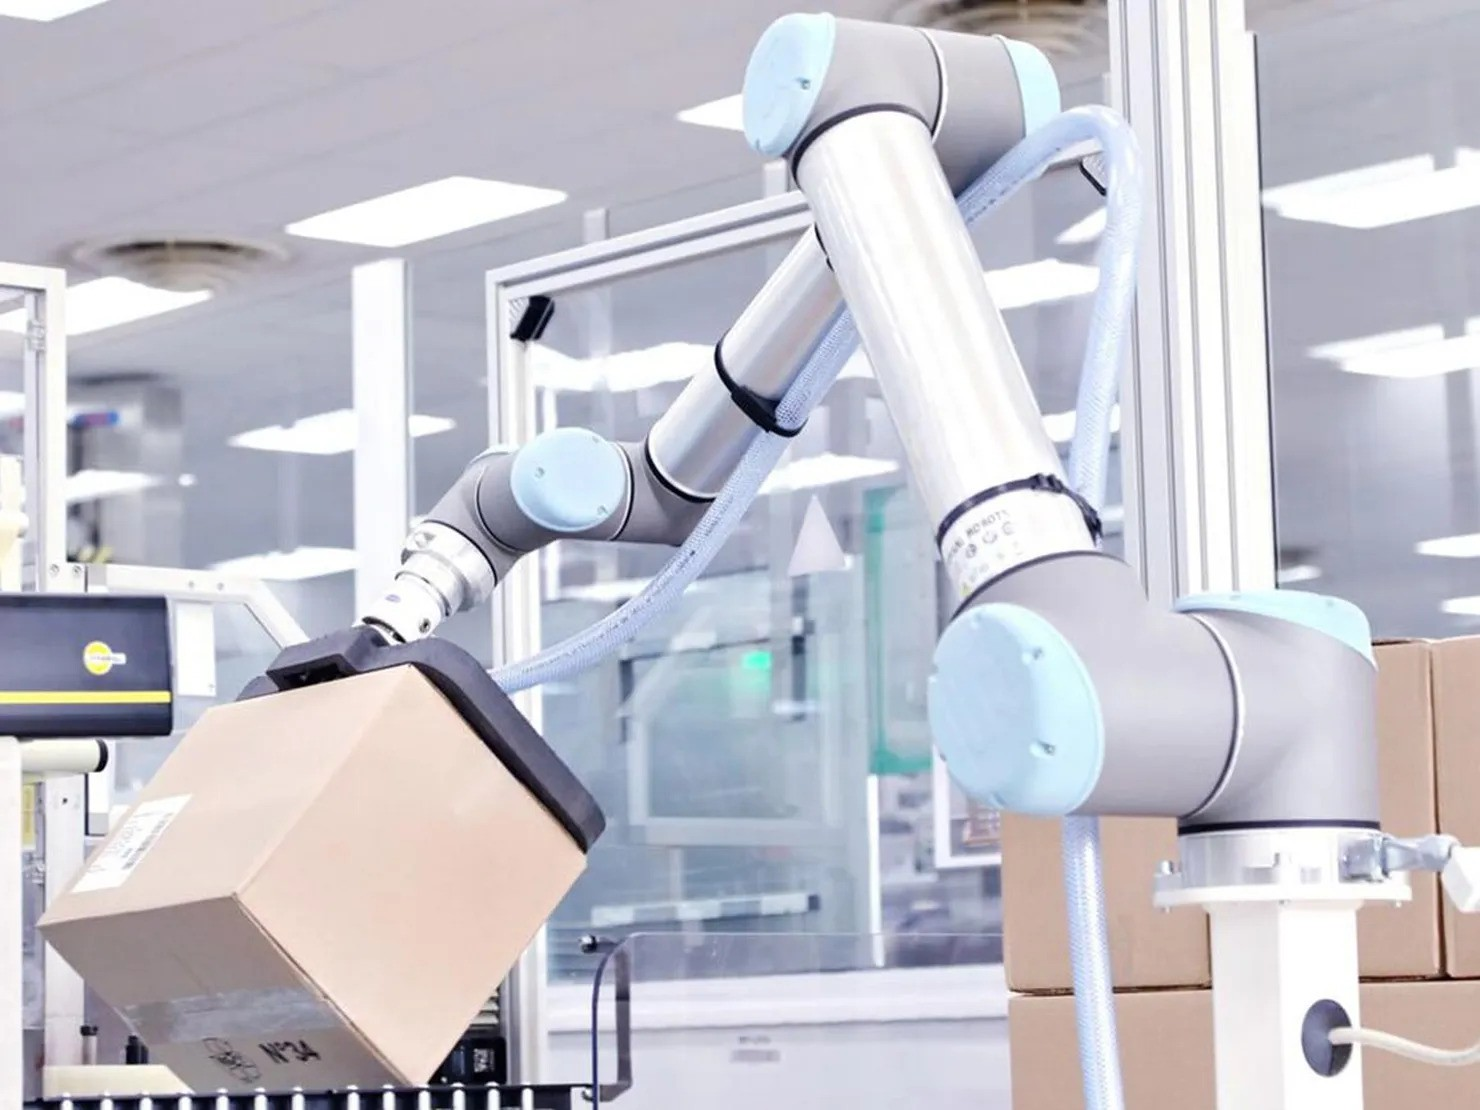
\includegraphics[width=0.5\linewidth]{Sections/2 Problemanalyse/Media/URrobot.jpg}
    \caption{UR5, et letvægt Cobot lavet i Danmark \parencite{2023URSeries}}
    \label{fig:ur5pic}
\end{figure}

\textit{Eksempel:} Universal Robots' UR-serie \parencite{2023URSeries}. Designet til at være flexible, billig og let. Primært tænkt til at "samle op, flytte, placere". Fx kan den placere en del foran et mennesker, der kan udføre noget arbejde, hvorefter UR5 kan flytte den væk igen. Cobots bruges altså til at automatisere "simple" handlinger hvorimod mennesker stadig udføre mere kompliceret arbejde.




\begin{comment}
Bruger subset af hele objektet 

Flytter firkant indtil det passer med det deformerede billede 

1 pixel giver 256 muligheder for subset - værdien har noget med bit at gøre. Gray level er 0 til 256. 

20x20 pixels giver 20x20x256=102400 muligheder for forskellige subsets. Hvis der er variation i værdierne 

Opsættes i en matrix, hvor 1 pixels er repræsenteret af en værdi (ofte fra 0 - 256). Forsøger at finde matrixen igen efter deformation. 

Små subsets, hvis vi vil finde flere forskydninger på et mindre område. 

Gælder om, at få små subsets, med små prikker.  

Mindre variation ved store prikker. 

Idéen med, at vi tager en firkant -> deformere -> prøver at genfinde firkanten.   
\end{comment}
 
